\documentclass[main.tex]{subfiles}
\begin{document}

\subsection{No shock accretion}

\marginpar{Wednesday\\ 2020-12-16, \\ compiled \\ \today}

% Yesterday we discussed column accretion onto a magnetized NS. 

If there is no shock, the velocity of the infalling gas will be very high
%
\begin{align}
v \sim v _{\text{free-fall}} = \sqrt{ \frac{2GM}{R}} \sim \num{.5} c
\,,
\end{align}
%
while if there is a collisionless shock the velocity will be much lower: \(v \ll c_s\).

The matter, with particles of mass \(m_1 \) (typically \(m_1 = m_p\)) accretes with a velocity \(u\) onto a plasma, which we assume to be composed of constituents with masses \(m_2 \) (typically \(m_2 = m_e\)) and \(m_1\).
We assume that the typical kinetic energy of an accreting particle is much larger than the thermal energy of the plasma on the surface:
%
\begin{align}
\frac{1}{2 } m_1 u^2 \gg \frac{3}{2} k_B T = \frac{1}{2} m_2 v_2^2
\,.
\end{align}

% \todo[inline]{Not \((\gamma -1 ) mc^2\)?}

The typical \textbf{deflection timescale} for the infalling particles will look like 
%
\begin{align}
t_D = \frac{v^2}{\dv{(\Delta v)^2}{t}}
\,,
\end{align}
%
(we take the square in order to have a positive quantity)  which can be calculated to be 
%
\begin{align}
t_D = \frac{m_1^2 u^3}{8 \pi n e_1^2 e_2^2 \log \Lambda }
\,,
\end{align}
%
where \(e_i\) are the charges of the particles, while \(\log \Lambda \) is known as the Coulomb logarithm. It is typically of the order \(\log \Lambda \sim 15 \divisionsymbol 20\), and it is given by 
%
\begin{align}
\log \Lambda = \log( \frac{\chi _{\text{max}}}{\chi _{\text{min}}})
\,,
\end{align}
%
where the \(\chi \)s are the maximum and minimum deflection angles in a collision, respectively.
% \todo[inline]{What are the \(e_i\)?}

This is the typical time required in order to isotropize an initially anisotropic velocity distribution --- it need not become compatible with the thermal velocity distribution. 
For that, we have a new \textbf{energy exchange timescale}: 
%
\begin{align}
t_E &= \frac{E^2}{\dv{(\Delta E)^2}{t}} \\
&= \underbrace{\frac{m_1^2u^3}{8 \pi n e_1^2 e_2^2 \log \Lambda }}_{t_D} \underbrace{\frac{m_2 u^2}{2 k_B T}}_{\gg 1} 
\,.
\end{align}

This is the time we need to wait for in order to reach a Maxwell-Boltzmann-like distribution. 

The last timescale we will introduce is the \textbf{slowing-down} timescale: the typical time needed for an incoming particle to become stationary with respect to the Neutron Star,
%
\begin{align}
t_S = \frac{u}{\dv{u}{t}} = \underbrace{\frac{m_1^2u^3}{8 \pi n e_1^2 e_2^2 \log \Lambda }}_{t_D} \underbrace{\frac{m_2}{m_1 + m_2 }}_{\sim 1/2000}
\,.
\end{align}

The slowing down is \emph{mostly} due to interactions between the incoming protons (\(m_1 \)) and the plasma electrons (\(m_2 \)).


% Typically, \(m_1 \sim m_p\) while \(m_2 \sim m_e\). 

% Then, 
% %
% \begin{align}
% t_S \propto \frac{m_e}{m_p + m_e} \sim \frac{m_e}{m_D} 
% \,,
% \end{align}
% %
% so \(t_S \sim t_D (m_e / m_p) \ll t_D\). 

The result we get is then \(t_S \ll t_D \ll t_E\) typically: first the particles slow down, then they isotropize, then they transfer their energies.

What happens, instead, if we take \(m_1 \) to be the \emph{electron} mass? Then, the stopping timescale will have contribution both from interactions with the plasma electrons and protons --- the contributions are \(m_e / (m_e + m_e) = 1/2\) and \(m_p / (m_p + m_e) \approx 1\) respectively, so they are both relevant. In this case, then, \(t_S \approx t_D \ll t_E\). 
A sketch of this is shown in figure \ref{fig:timescales}.

\begin{figure}[]
\centering
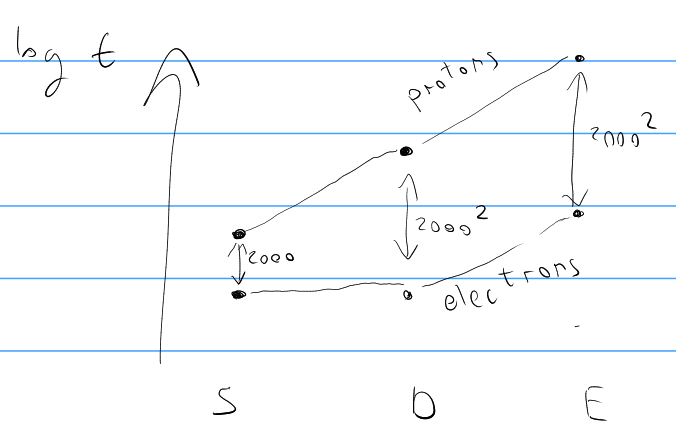
\includegraphics[width=\textwidth]{figures/timescales}
\caption{A very bad figure to show how the timescales look.}
\label{fig:timescales}
\end{figure}

% Electrons are decelerated in the same way by both electrons and protons, protons are mostly decelerated by electrons: 
% %
% \begin{align}
% t_S^{(p)} &\propto \frac{m_p}{m_e + m_p} \\
% t_S^{(e)} &\propto 1
% \,.
% \end{align}

The stopping length will typically be \(\lambda _S \sim u t_S\), and the path will look like a random walk. We can write this in terms of the kinetic energy of the proton: \(E_{kp} = m_p u^2 /2\), so  
%
\begin{align}
\lambda _S = \frac{E_{kp}^2}{2 \pi n e^4 \log \Lambda } \frac{m_e}{m_p} = \frac{E^2_{kp}}{2 \pi \rho e^{4} \log \Lambda } m_e
\,.
\end{align}

The stopping column density is defined as \(y_0 = \rho \lambda _S\), which resembles the definition for the optical depth (but without the absorption coefficient). Dimensionally, it is a mass over a length squared. 

The plasma will start to emit photons as it is heated by the accretion, and it is interesting to compare the typical free path of a photon to \(\lambda _S\). The main source of opacity will be scattering;
the Thompson cross-section is given by 
%
\begin{align}
\sigma _T = \frac{8 \pi }{3} \frac{e^{4}}{m_e^2 c^{4}}
\,.
\end{align}


The mean free path for photons looks like \(\lambda _{ph} = 1/ (n \sigma _T)\). The ratio \(\lambda _S / \lambda  _{\text{ph}}\) is then 
%
\begin{align}
\frac{\lambda_S}{\lambda_{\text{ph}}} = \frac{m_p}{m_e} \frac{1}{3 \log \Lambda } \qty( \frac{u}{c})^4
\,;
\end{align}
%
in order for the accreting material to ``penetrate'' the plasma and heat it from inside, as opposed to losing all of its energy on the surface, we need to ask \(\lambda _S > \lambda  _{\text{ph}}\),
and this is equivalent to \(u/c \gtrsim \num{.4}\).

\end{document}
